% !TeX root = digital_signatures.tex
\documentclass{beamer}
\usepackage[spanish]{babel}
\usepackage{amsmath}
\usepackage{amsfonts}
\usepackage{booktabs}

\usetheme{Madrid}

\setbeamertemplate{navigation symbols}{}

\author{Pedro Palacios Almendros}
\title{Firmas digitales DSA y ElGamal}
\institute[UCM]{
    Álgebra Computacional \\
    Universidad Complutense de Madrid
}

\begin{document}

\makeatletter
\setbeamertemplate{footline}
{
  \leavevmode%
  \hbox{%
  \begin{beamercolorbox}[wd=.333333\paperwidth,ht=2.25ex,dp=1ex,center]{author in head/foot}%
    \usebeamerfont{author in head/foot}\insertshortauthor%~~\beamer@ifempty{\insertshortinstitute}{}{(\insertshortinstitute)}
  \end{beamercolorbox}%
  \begin{beamercolorbox}[wd=.333333\paperwidth,ht=2.25ex,dp=1ex,center]{title in head/foot}%
    \usebeamerfont{title in head/foot}\insertshorttitle
  \end{beamercolorbox}%
  \begin{beamercolorbox}[wd=.333333\paperwidth,ht=2.25ex,dp=1ex,right]{date in head/foot}%
    \usebeamerfont{date in head/foot}\insertshortdate{}\hspace*{2em}
    \insertframenumber{} / \inserttotalframenumber\hspace*{2ex} 
  \end{beamercolorbox}}%
  \vskip0pt%
}
\makeatother

\frame{\titlepage}

\AtBeginSection[]
{
  \begin{frame}
    \frametitle{\insertsectionhead}
    \tableofcontents[currentsection]
  \end{frame}
}

\section{Firmas digitales}

\begin{frame}
    \frametitle{Firmas digitales: Motivación}

    Muchas aplicaciones requieren poder \alert{verificar la autenticidad} de un mensaje:

    \begin{itemize}
        \item Trámites oficiales con la administración pública
        \item Firma de contratos electrónicos
        \item Verificación de la integridad de archivos y descargas
    \end{itemize}
    
\end{frame}

\subsection{Propiedades}

\begin{frame}
    \frametitle{Firmas digitales: Propiedades}

    \begin{block}{Definición}
        Una \alert{firma digital} es un mecanismo criptográfico que permite al receptor de un mensaje firmado digitalmente identificar al emisor de dicho mensaje y cumple las siguientes propiedades:
    \end{block}

    \begin{itemize}
        \item \textbf{Infalsificable}. Las firmas deben poder ser generadas solamente por el firmante.
        \item \textbf{Inalterable}. La firma digital confirma que el mensaje no ha sido alterado. Si se altera el mensaje, la firma deja de ser válida.
        \item \textbf{No repudiable}. Una vez realizada la firma, el firmante no puede \textit{echarse atrás} e invalidarla.
        \item \textbf{Verificable}. Las firmas deben ser fácilmente verificables por los receptores de las mismas.
    \end{itemize}
    
\end{frame}

\subsection{Funciones hash}

\begin{frame}
    \frametitle{Funciones hash}

    \begin{block}{Definición}
        Una \alert{función hash} es una función de un conjunto de tamaño de entrada (cadenas) a un conjunto de tamaño fijo de salida con las siguientes propiedades:
    \end{block}

    \begin{itemize}
        \item \textbf{Uniformidad}. Todos los elementos del conjunto de salida deberían tener relativamente la misma probabilidad.
        \item \textbf{Eficiencia}. Calcular la función hash de una cadena de entrada debe ser rápido.
        \item \textbf{Irreversibilidad}. No debe ser factible obtener (una o varias) cadenas cuya imagen sea cierto elemento dado.
        \item \textbf{Determinismo}. La función hash de una cadena debe ser siempre la misma.
    \end{itemize}
    
\end{frame}

\begin{frame}
    \frametitle{Funciones hash}

    Las funciones hash \alert{resumen} una cadena de ancho variable en un valor de un conjunto finito de tamaño fijo (por ejemplo un elemento de $\mathbb{Z}/n\mathbb{Z}$).

    \begin{figure}
        \centering
        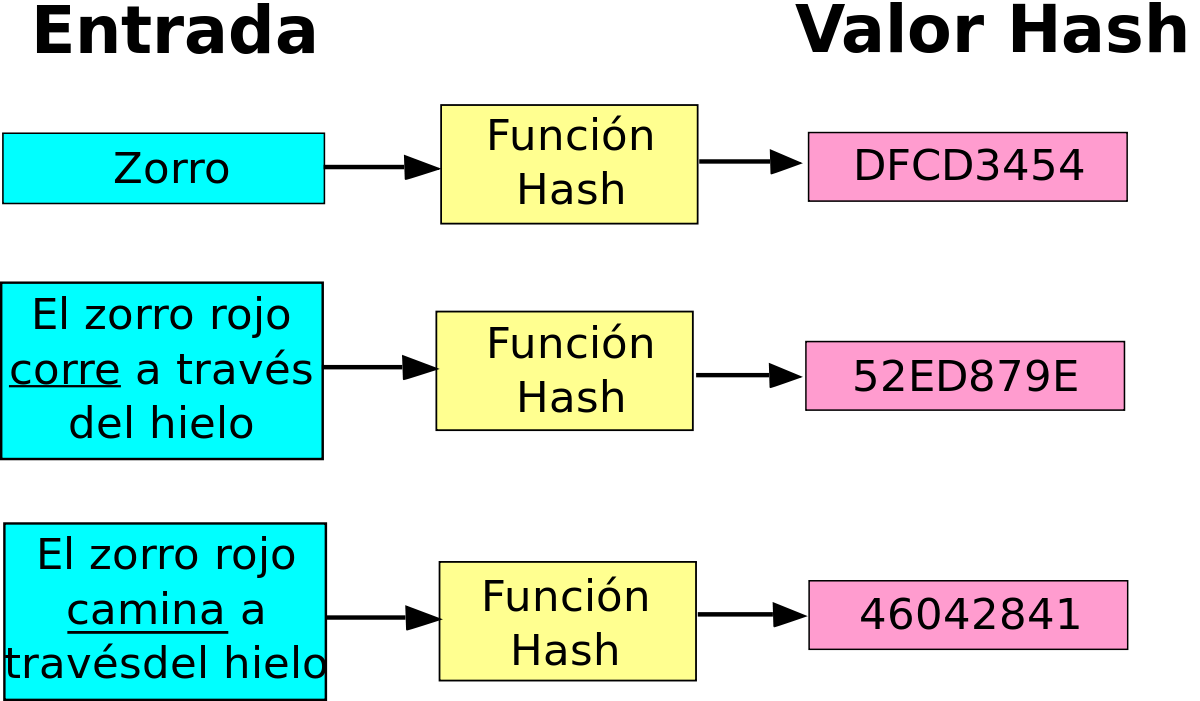
\includegraphics[width=0.7\textwidth]{Hash.png}
    \end{figure}


    Las cadenas hash pueden usarse para verificar la integridad de un mensaje. Si el mensaje cambia un poco, su hash cambiará sustancialmente.
\end{frame}

\subsection{Claves pública y privada}

\begin{frame}
    \frametitle{Claves pública y privada}

    \begin{figure}
        \centering
        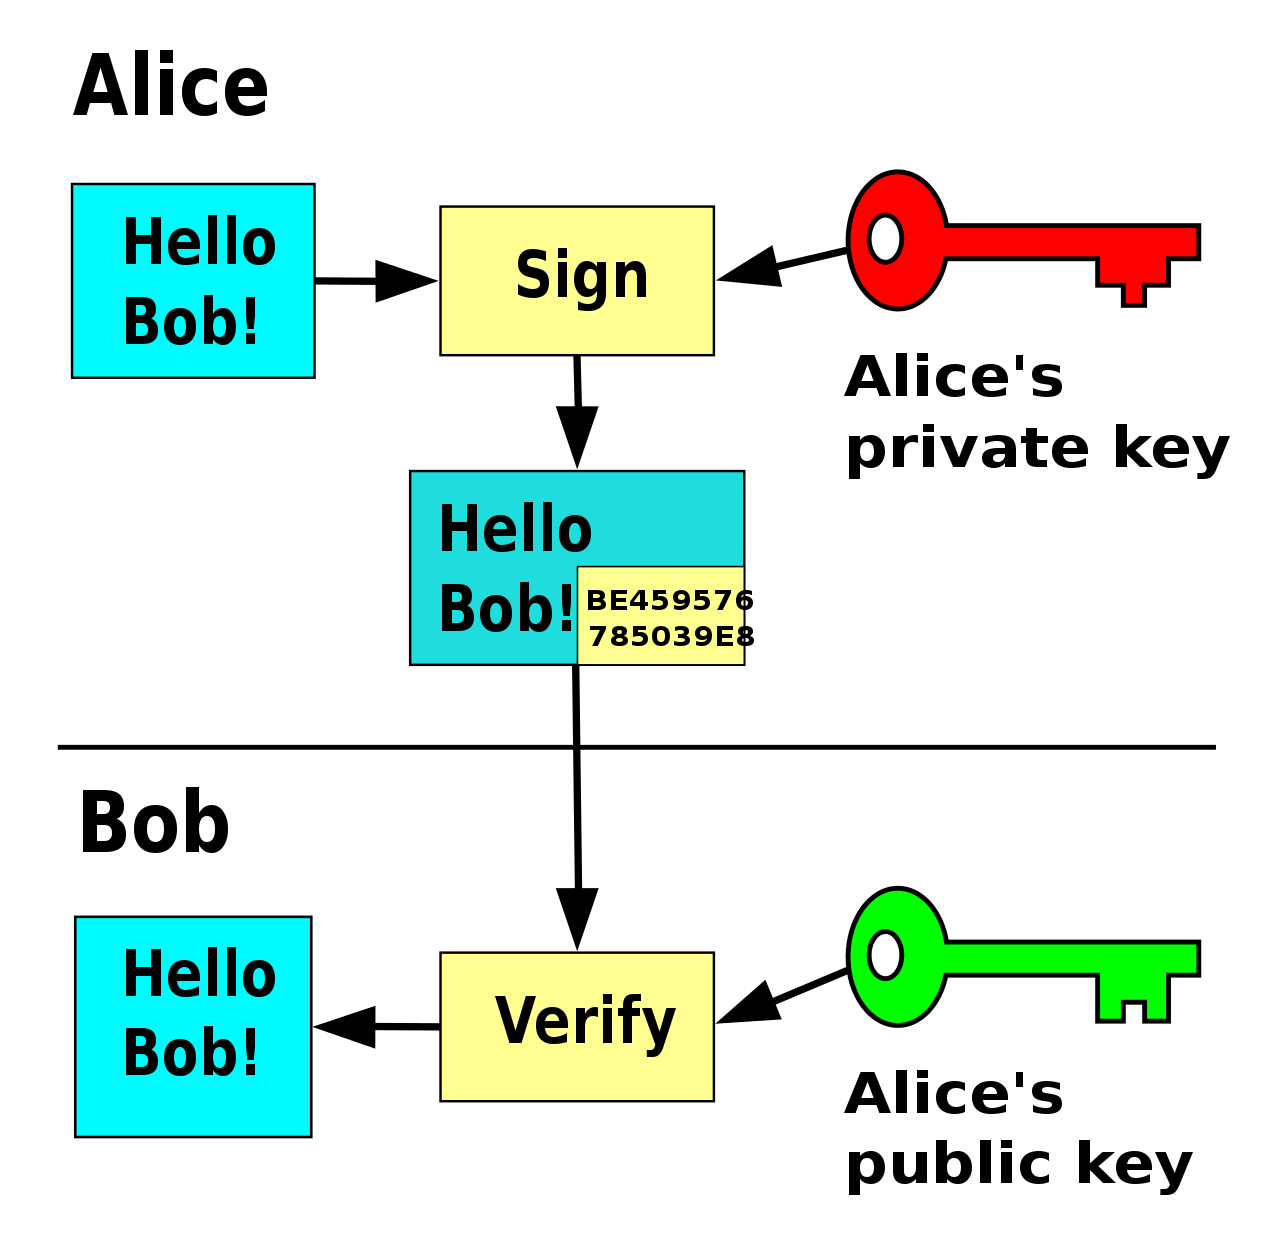
\includegraphics[width=0.35\textwidth]{PrivateKeySign.png}
    \end{figure}

    El emisor tiene dos claves (una pública y una privada) que se utilizan de forma dual para firmar y verificar:

    \begin{itemize}
        \item La \textbf{clave privada} solo la conoce el emisor, y la utiliza para firmar el mensaje digitalmente.
        \item La \textbf{clave pública} se publica a todo el mundo, y cualquiera la puede utilizar para verificar el mensaje.
    \end{itemize}
    

\end{frame}


\section{ElGamal}

\subsection{Firma y verificación}

\begin{frame}
    \frametitle{ElGamal: Protocolo de firma y verificación}

    El protocolo para firmar y verificar un mensaje consiste en los siguientes pasos:
    \begin{enumerate}
        \item Generación de parámetros compartidos por todos los usuarios del sistema
        \item Generación de claves diferentes para cada usuario del sistema
        \item Distribución de las claves públicas entre los usuarios
        \item Firma por parte del emisor del mensaje
        \item Verificación por parte del receptor
    \end{enumerate}
\end{frame}

\begin{frame}
    \frametitle{ElGamal: Generación de parámetros}

    Se eligen parámetros que serán compartidos por todos los usuarios del sistema.

    \begin{enumerate}
        \item Se elige un tamaño de clave $N$
        \item Se elige un número primo $p$ de $N$ bits
        \item Se elige una función hash $H$ cuyo conjunto de salida son los enteros de $L$ bits, con $L \le N$
        \item Se elige un generador $g < p$ del grupo multiplicativo de los enteros módulo $p$, ${\left(\mathbb{Z}/p\mathbb{Z} \right)}^{*}$.
    \end{enumerate}

    Los parámetros del protocolo son $(p, H, g)$.
\end{frame}

\begin{frame}
    \frametitle{ElGamal: Generación y distribución de claves}

    Dados los parámetros del sistema, se elige una clave privada y una pública distintas para cada usuario.

    \begin{enumerate}
        \item Se escoge aleatoriamente $x \in \left\{1, ..., p-2\right\}$.
        \item Calculamos $y := g^x \mod p$ usando exponenciación modular.
    \end{enumerate}

    La \textbf{clave privada} es $x$, la \textbf{clave pública} es $y$.
    \\[10pt]
    Nótese que para obtener la clave privada desde la clave pública habría que resolver el problema del \alert{logaritmo discreto}, para el que no se conoce ninguna implementación efectiva para el caso general.
    \\[10pt]
    Únicamente la \textbf{clave pública} se distribuye a todos los usuarios, la clave privada se mantiene secreta.
\end{frame}


\begin{frame}
    \frametitle{ElGamal: Firma}

    Supongamos que tenemos un mensaje $m$ que queremos firmar:

    \begin{enumerate}
        \item Elegimos un entero $k \in \left\{2, ..., p-2\right\}$ tal que $k$ sea coprimo con $p-1$ 
        \item Calculamos $r := g^k \mod p$ usando exponenciación modular
        \item Computamos $k^{-1} \mod \left(p-1\right)$ utilizando el algoritmo extendido de Euclides, que existe pues $\gcd(k, p-1) = 1$
        \item Computamos $$s := \left( H(m) - x \cdot r  \right) \cdot k^{-1} \mod \left(p-1\right)$$
        \item En el caso improbable de que $s=0$, empezamos de nuevo con otro $k$ aleatorio
    \end{enumerate}

    El resultado del proceso es la firma digital, que será la tupla $(r, s)$.

\end{frame}

\begin{frame}
    \frametitle{ElGamal: Verificación}

    Para verificar que una firma $(r, s)$ es válida para un mensaje $m$ hacemos la siguiente comprobación:
    \begin{enumerate}
        \item Comprobamos que $0 < r < p$ y que $0 < s < p-1$
        \item La firma será válida si y sólo si $$ g^{H(m)} \equiv y^r \cdot r^s \mod p$$
    \end{enumerate}

\end{frame}

\subsection{Corrección}

\begin{frame}
    \frametitle{ElGamal: Corrección}

    Demostremos que el algoritmo es correcto, es decir, que una firma generada por el algoritmo de verificación será aceptada por el verificador.

    \begin{itemize}
        \item Recordamos la definición de $s$ en la firma $$s := \left( H(m) - x \cdot r  \right) \cdot k^{-1} \mod \left(p-1\right)$$
        \item Multiplicando por $k$ y despejando, se tiene que $$ H(m) \equiv x r + s k  \mod \left(p-1\right) $$
        \item Como $g$ es generador de ${\left(\mathbb{Z}/p\mathbb{Z} \right)}^{*}$, tiene orden $\phi(p)=p-1$, por lo que $g^{\alpha} \equiv g^{\alpha \mod \left(p-1\right)} \mod p$. Aplicando esto:
        \begin{align*}
            g^{H(m)} & \equiv g^{x r + s k} \mod p  \\
                     & \equiv \left(g^{x}\right)^r \left(g^k\right)^s \mod p \\
                     & \equiv \left(y\right)^r \left(r\right)^s \mod p
        \end{align*}
    \end{itemize}    
\end{frame}

\subsection{Ejemplo}

\begin{frame}
    \frametitle{ElGamal: Ejemplo}
    \begin{itemize}
        \item Supongamos que los parámetros del sistema son $p = 13$, $H(m) = m$, $g = 2$.
        \item Supongamos que el usuario elige la clave privada $x = 3$, por lo que su clave pública será $y := g^x \mod p \equiv 2^3  \mod 13 \equiv 8 \mod 13$.
        \item Supongamos que queremos firmar el mensaje $m = 11$ y elegimos $k=5$ ($\gcd(k, p-1)=\gcd(5, 12)=1$):
        \begin{itemize}
            \item $r := g^k \mod p \equiv 2^5 \mod 13 \equiv 32 \mod 13 \equiv 6 \mod 13$
            \item Con el algoritmo extendido de Euclides hallamos que $5 \cdot 5 -2 \cdot 12 = 1$, por lo que $k^{-1} \equiv 5 \mod 12$
            \item $s := \left( H(m) - x \cdot r  \right) \cdot k^{-1} \mod \left(p-1\right) \equiv \left( 11 - 3 \cdot 6  \right) \cdot 5 \mod 12 \equiv 1 \mod 12 $
        \end{itemize}
        \item La firma es por tanto $(r, s) = (6, 1)$. Verifiquemos que es correcta:    
        \begin{itemize}
            \item $g^{H(m)} \mod p \equiv 2^{11} \mod 13 \equiv 2048 \mod 13 \equiv 7 \mod 13 $
            \item $\left(y\right)^r \left(r\right)^s \mod p = 8^6 \cdot 6^1 \mod 13 \equiv 1572864 \mod 13 \equiv 7 \mod 13 $
        \end{itemize}
    \end{itemize}    
\end{frame}

\subsection{Seguridad}

\begin{frame}
    \frametitle{ElGamal: Seguridad}

    La seguridad de ElGamal radica en la dificultad de resolver ciertos problemas que se consideran difíciles:
    \begin{itemize}
        \item Hallar la clave privada usando la clave pública. Requiere resolver el problema del logaritmo discreto: $y := g^x \mod p$.
        \item Encontrar colisiones en la función hash: $H(m) = H(M) \mod \left(p-1\right) $
        \item Falsificar firmas: dados $(g, m, y, p)$, encontrar $(r, s)$ tal que $g^{H(M)} \equiv y^r r^s \mod p$
        \begin{itemize}
            \item Si se fija $r$ y se intenta despejar $s$, el problema es equivalente a resolver el logaritmo discreto.
            \item Si se fija $s$ y se intenta despejar $r$, no se ha demostrado que el problema sea NP, pero tampoco se ha encontrado una solución eficiente.
            \item Tampoco se ha encontrado un algoritmo eficiente para despejar $(r, s)$ a la vez.
        \end{itemize}
    \end{itemize}
\end{frame}

\begin{frame}
\frametitle{ElGamal: Ataques}

\begin{itemize}
    \item  Si se usa la misma $k$ para dos mensajes distintos, podríamos obtener la clave privada $x$ resolviendo el sistema de ecuaciones lineales:

    \[
        \left\{ \begin{array}{lll}
            H(m_1)&\equiv&x \cdot r_1 + s_1 \cdot k \mod \left(p-1\right) \\
            H(m_2)&\equiv&x \cdot r_2 + s_2 \cdot k \mod \left(p-1\right)
        \end{array}  \right.
    \]
    El sistema tiene dos ecuaciones y dos incógnitas ($x$ y $k$), el resto son datos conocidos.

    \item Generar firmas para ciertos mensajes derivados a partir de una firma valida (si $H(M) = M$):
    \begin{itemize}
        \item Si un emisor legítimo firma un mensaje $M$, seleccionando arbitrariamente $A$, $B$, $C$ arbitrariamente tal que $\gcd(Ar – Cs, p-1)=1$, entonces se puede ver que $(r', s')$ firma $m'$ donde
            \begin{align*}
                r' & \equiv r^A g^B y^C \mod p \\
                s' & \equiv \frac{s r'}{Ar - Cs} \mod \left(p-1\right) \\
                m' & \equiv \frac{r' \left( Am + Bs \right) }{Ar - Cs} \mod \left(p-1\right)
            \end{align*}
    \end{itemize}
\end{itemize}

\end{frame}

\section{DSA}

\subsection{Firma y verificación}

\begin{frame}
    \frametitle{DSA: Generación de parámetros}

    Se eligen parámetros que serán compartidos por todos los usuarios del sistema.

    \begin{enumerate}
        \item Se elige una función hash $H$ con tamaño de salida $|H|$.
        \item Se elige un tamaño de clave $L$. Originalmente $L$ era un múltiplo de 64 entre 512 y 1024.
        \item Se elige un tamaño del módulo $N < L$. Si $N < |H|$, tomamos únicamente los últimos $N$ bits de la función hash. Originalmente $(L, N) \in \left\{ (1024, 160), (2048, 224), (2048, 256), (3072, 256) \right\}$ 
        \item Se elige un primo $q$ de $N$ bits
        \item Se elige un primo $p$ de $L$ bits tal que $q \vert \left(p-1\right)$
        \item Se elige $h \in \left\{2, ..., p-2\right\}$. Usualmente $h = 2$ 
        \item Se elige $g := h^{\frac{p-1}{q}} \mod p$. En el caso improbable de que $g=1$, se elige otro $h$ distinto.
    \end{enumerate}

    Los parámetros del protocolo son $(p, q, H, g)$.
\end{frame}

\begin{frame}
    \frametitle{DSA: Generación y distribución de claves}

    Dados los parámetros del sistema, se elige una clave privada y una pública distintas para cada usuario.

    \begin{enumerate}
        \item Se escoge aleatoriamente $x \in \left\{1, ..., q-1\right\}$.
        \item Calculamos $y := g^x \mod p$ usando exponenciación modular.
    \end{enumerate}

    La \textbf{clave privada} es $x$, la \textbf{clave pública} es $y$.
    \\[10pt]
    Nótese que al igual que en ElGamal, para obtener la clave privada desde la clave pública habría que resolver el problema del \alert{logaritmo discreto}, para el que no se conoce ninguna implementación efectiva para el caso general.
    \\[10pt]
    De nuevo, únicamente la \textbf{clave pública} se distribuye a todos los usuarios, la clave privada se mantiene secreta.
\end{frame}

\begin{frame}
    \frametitle{DSA: Firma}

    Supongamos que tenemos un mensaje $m$ que queremos firmar:

    \begin{enumerate}
        \item Elegimos un entero $k \in \left\{1, ..., q-1\right\}$ 
        \item Calculamos $r := \left(g^k \mod p\right) \mod q$. En el caso improbable de que $r=0$, empezar de nuevo con otro $k$.
        \item Computamos $k^{-1} \mod q$ utilizando el algoritmo extendido de Euclides, que existe pues $q$ es primo.
        \item Computamos $$s := \left( k^{-1} \left( H(m) + x r  \right) \right) \mod q$$
        \item En el caso improbable de que $s=0$, empezamos de nuevo con otro $k$ aleatorio
    \end{enumerate}

    El resultado del proceso es la firma digital, que será la tupla $(r, s)$.

\end{frame}

\begin{frame}
    \frametitle{DSA: Verificación}

    Para verificar que una firma $(r, s)$ es válida para un mensaje $m$ hacemos la siguiente comprobación:
    \begin{enumerate}
        \item Comprobamos que $0 < r < q$ y que $0 < s < q$
        \item Calculamos $w = s^{-1} \mod q$
        \item Calculamos $u_1 = H(m)w \mod q$
        \item Calculamos $u_2 = r \cdot w \mod q$
        \item Calculamos $v = \left( g^{u_1} y^{u_2} \mod p \right) \mod q$
        \item La firma será válida si y sólo si $v \equiv r \mod q$
    \end{enumerate}

\end{frame}

\begin{frame}
    \frametitle{DSA: Corrección (1)}

    Demostremos que el algoritmo es correcto, es decir, que una firma generada por el algoritmo de verificación será aceptada por el verificador.

    \begin{itemize}
        \item Primero notamos que como $g = h^{\frac{p-1}{q}} \mod p$, aplicando el pequeño teorema de Fermat, $g^q \equiv h^{p-1} \equiv 1 \mod p$. Por tanto, $g$ tiene orden $\le q$. Como $g > 1$ y $q$ es primo y el orden de $g$ divide a $q$, entonces $g$ tiene orden $q$.
        \item El firmante calculó $$s := \left( k^{-1} \left( H(m) + x r  \right) \right) \mod q$$ Como $s \not\equiv 0 \mod q$, $\exists s^{-1}$, podemos despejar $k$:
        \begin{align*}
            k & \equiv H(m) s^{-1} + x r s^{-1} \mod q  \\
              & \equiv H(m) w + x r w \mod q
        \end{align*}
        
        \item Como $g$ tiene orden $q$
        \begin{align*}
            g^k & \equiv g^{H(m) w} g^{x r w} \mod p  \\
              & \equiv g^{H(m) w} y^{r w} \mod p
        \end{align*}
    \end{itemize}    
\end{frame}


\subsection{Corrección}

\begin{frame}
    \frametitle{DSA: Corrección (2)}

    \begin{itemize}
        \item Hemos visto que
        \begin{align*}
            g^k & \equiv g^{H(m) w} y^{r w} \mod p    \\
              & \equiv g^{u_1} y^{u_2} \mod p
        \end{align*}

        \item Por último, vemos que
        \begin{align*}
            r & \equiv \left( g^k \mod p \right) \mod q    \\
              & \equiv \left( g^{u_1} y^{u_2} \right) \mod p \\
              & \equiv v \mod q
        \end{align*}


    \end{itemize}    
\end{frame}

\subsection{Ejemplo}

\begin{frame}
    \frametitle{DSA: Ejemplo (1)}

    \begin{itemize}
        \item Supongamos que los parámetros del sistema son $p = 283$, $q = 47$, $H(m) = m$, $g = 60$. Se tiene que $p-1 = 282 = 6 \cdot 47 = 6q$.
        \item Supongamos que el usuario elige la clave privada $x = 24$, por lo que su clave pública será $y := g^x \mod p \equiv 60^{24}  \mod 283 \equiv 158 \mod 283$.
        \item Supongamos que queremos firmar el mensaje $m = 41$ y elegimos $k=15$:
        \begin{itemize}
            \item $t = g^k \mod p \equiv 60^{15} \mod 283 \equiv 207 \mod 283$
            \item $r := t \mod q \equiv 207 \mod 47 \equiv 19 \mod 47$
            \item Con el algoritmo extendido de Euclides hallamos que $22 \cdot 15 -7 \cdot 47 = 1$, por lo que $k^{-1} \equiv 22 \mod 47$
            \item $s :=  k^{-1} \left( H(m) + x \cdot r  \right) \mod q \equiv 22 \cdot \left( 41 + 24 \cdot 19  \right) \mod 47 \equiv 30 \mod 47 $
        \end{itemize}

        \item La firma es por tanto $(r, s) = (19, 30)$.
    \end{itemize}    
\end{frame}

\begin{frame}
    \frametitle{DSA: Ejemplo (2)}
    
    \begin{itemize}
        \item Los parámetros del sistema son $p = 283$, $q = 47$, $H(m) = m$, $g = 60$.
        \item La clave privada $x = 24$, y la clave pública es $y := 158 \mod 283$.
        \item Verifiquemos ahora que la firma $(r, s) = (19, 30)$ del mensaje $m=41$ es correcta:
        \begin{itemize}
            \item Con el algoritmo extendido de Euclides hallamos que $11 \cdot 30 -7 \cdot 47 = 1$, por lo que $w := s^{-1} \mod q \equiv 11 \mod 47$
            \item $u_1 := H(m) w \mod q \equiv 41 \cdot 11 \mod 47 \equiv 28 \mod 47 $
            \item $u_2 := r w \mod q \equiv 19 \cdot 11 \mod 47 \equiv 21 \mod 47 $
            
            \item Calculamos $v$:
            \begin{align*}
                v & := \left(g^{u_1} y^{u_2} \mod p \right) \mod q \\ 
                & \equiv \left(60^{28} \cdot 158^{21} \mod 283 \right) \mod 47 \\
                & \equiv 207 \mod 47 \\
                & \equiv 19 \mod 47
            \end{align*}
            \item Comprobamos que efectivamente, $v \equiv 19 \equiv r \mod 47$
        \end{itemize}
    \end{itemize}
\end{frame}

\subsection{Seguridad}

\begin{frame}
    \frametitle{DSA: Seguridad}

    Al igual que en ElGamal, la seguridad de DSA radica en la dificultad de resolver ciertos problemas que se consideran difíciles:
    \begin{itemize}
        \item Hallar la clave privada usando la clave pública. Requiere resolver el problema del logaritmo discreto: $y := g^x \mod p$.
        \item Encontrar colisiones en la función hash: $H(m) = H(M) \mod \left(p-1\right) $
        \item Falsificar firmas: dados $(g, m, y, p)$, encontrar $(r, s)$ tal que 
        $$r = \left( g^{\left( H(m) \cdot s^{-1} \bmod q  \right)} y^{\left( r \cdot s^{-1} \bmod q  \right)} \mod p \right) \bmod q$$
        \begin{itemize}
            \item No se conoce ningún algoritmo eficiente para poder despejar $(r, s)$. 
            
        \end{itemize}
    \end{itemize}

\end{frame}

\begin{frame}
    \frametitle{DSA: Ataques}

    En DSA es muy importante que el valor de \alert{$k$ sea totalmente aleatorio} y no sea predecible.

    \begin{itemize}
        \item Se descubrió la clave privada (ECDSA) que Sony usaba para firmar los programas de la Play Station 3 debido a que se reusaba siempre el mismo $k$.
        \item Si se usa el mismo $k$ en dos firmas distintas, entonces:
        \[
            \left\{ \begin{array}{lll}
                s_1 & \equiv & \left( k^{-1} \left( H(m_1) + x r_1  \right) \right) \mod q \\
                s_2 & \equiv & \left( k^{-1} \left( H(m_2) + x r_2  \right) \right) \mod q
            \end{array}  \right.
        \] 
        Que se puede reescribir en el siguiente sistema lineal:

        \[
            \left\{ \begin{array}{lll}
                k s_1 - x r_1 & \equiv & H(m_1) \mod q \\
                k s_2 - x r_2 & \equiv & H(m_2) \mod q
            \end{array}  \right.
        \] 
        Como $\mathbb{Z}/q{\mathbb{Z}}$ es un cuerpo, podemos despejar $(k, x)$ utilizando el método de Gauss.
    \end{itemize}

\end{frame}


\begin{frame}
    \frametitle{Comparación entre ElGamal y DSA}

    \begin{itemize}
        \item Hoy en día se utiliza sobre todo DSA en vez de ElGama, por motivos de eficiencia.
        \item En DSA trabajamos con dos primos $p$ y $q$. La clave pública tiene la resistencia al logaritmo discreto de $p$ (que suele ser grande). Sin embargo, la mayor parte de las operaciones se realizan módulo $q$ (en ElGamal debemos realizar exponenciaciones modulares con exponentes de tamaño similar a $p$), y $q << p$. \\
        
        \begin{table}[]
            \begin{tabular}{ccc} \toprule
                {$\mathbf{\vert p \vert}$} & {$\mathbf{|q|}$} & {\textbf{Hash}} \\ \hline
                1024 & 160 & SHA-1 \\
                2048 & 224 & SHA-224 \\
                2048 / 3072 & 256 & SHA-256 \\ \bottomrule
            \end{tabular}
        \end{table}
        \item Además, las firmas $(r, s)$ de DSA son mucho más pequeñas que las de ElGamal, pues $r$, $s$ son enteros módulo $q$, en vez de serlo módulo $p$.
    \end{itemize}
\end{frame}

\section {Generación de parámetros}

\begin{frame}
    
    \frametitle{Generación de números primos}

    Para generar un número primo seguimos los siguientes pasos:
    \begin{enumerate}
        \item Fijamos $N$, el tamaño en bits del número primo.
        \item Generamos un número aleatorio $n$ entre $2^{n-1}+1$ y $2^{n}-1$, ambos inclusives.
        \item Forzamos que sea impar haciendo el bit menos significativo 1.
        \item Comprobamos si algunos primos pequeños ($<300$) precomputados con una criba de eratóstenes dividen a $n$. Si lo hacen, volvemos a elegir $n$.
        \item Ejecutamos el test de primalidad de Miller-Rabin (con 20 iteraciones). Si el test indica que $n$ un número compuesto, elegimos un nuevo $n$ y probamos de nuevo.
    \end{enumerate}

\end{frame}

\begin{frame}
    \frametitle{Generación de parámetros ElGamal}

    Para generar los parámetros de ElGamal, necesitamos generar un primo $p$ de $N$ bits y un generador $g$ de $\left( \mathbb{Z} / p \mathbb{Z} \right)^{*}$. Para facilitar la tarea de encontrar una raíz primitiva, vamos a dotar de cierta estructura a los $p$ generados:

    \begin{enumerate}
        \item Generamos un primo $q$ de tamaño $N-1$ bits.
        \item Computamos $p = 2q + 1$ y comprobamos si es primo. Si no lo es, volvemos a elegir $q$ aleatoriamente.
        \item Por el teorema de Lagrange, como $p-1 = 2 q$ con $q$ primo, los posibles órdenes de los elementos de $\left( \mathbb{Z} / p \mathbb{Z} \right)^{*}$ son 1, 2, $q$, $p-1$. Nótese que el único elemento de orden 2 es $p-1 \equiv -1 \mod p$ y el único elemento de orden 1 es la identidad. Habrá $\phi(q) = q - 1$ elementos de orden $q$, por lo que aproximadamente el 50\% de los elementos serán generadores.
        \item Elegimos aleatoriamente $g \in \left\{2, ..., p-2\right\}$. Si $g^q \not\equiv 1 \mod p$, hemos acabado y $g$ es un generador. En caso contrario, elegimos un nuevo $g$ aleatoriamente.
    \end{enumerate}

\end{frame}

\begin{frame}
    \frametitle{Generación de parámetros DSA}

    Para generar los parámetros de ElGamal, necesitamos generar un primo $q$ de $L$ bits y un primo $p$ de $N$ bits tal que $q \vert (p-1)$.
    \begin{itemize}
        \item Generamos un primo $q$ de tamaño $L$ bits.
        \item Generamos un número $m$ de $N-L$ bits.
        \item Comprobamos si $p = m q + 1$ es primo. Si no lo es, escogemos otro múltiplo $m$. Si tras muchos intentos con el mismo $q$ no encontramos ningún múltiplo, elegimos otro $q$.
    \end{itemize}

\end{frame}


\begin{frame}<handout:0>
    \frametitle{Preguntas}
    
    \centering
    \Huge ¿Alguna pregunta?

\end{frame}

\end{document}
